% Práctica 1 - Robótica Inteligente Aplicada - Memoria
% Compilar con pdfLaTeX (Carlito, equivalente a Calibri) o con XeLaTeX/LuaLaTeX (Calibri).
\documentclass[11pt,a4paper]{article}

\usepackage{iftex}
\ifPDFTeX
  \usepackage[T1]{fontenc}
  \usepackage[utf8]{inputenc}
  \usepackage[sfdefault,lining]{carlito}
\else
  \usepackage{fontspec}
  \IfFontExistsTF{Calibri}{\setmainfont{Calibri}}{\setmainfont{Carlito}}
\fi
\usepackage[spanish,es-noshorthands,es-tabla]{babel}
\usepackage[a4paper,margin=2cm]{geometry}
\usepackage{graphicx}
\usepackage{booktabs,tabularx}
\usepackage[font=small,labelfont=bf,skip=3pt]{caption}
\usepackage{enumitem}
\usepackage{titlesec}
\usepackage[colorlinks=true,linkcolor=blue]{hyperref}

\graphicspath{{../figuras/}{figuras/}}
\setlength{\parindent}{0pt}
\setlength{\parskip}{4pt}
\setlist{nosep,leftmargin=12pt}
\titleformat{\section}{\large\bfseries}{\thesection.}{0.4em}{}
\titleformat{\subsection}{\normalsize\bfseries}{\thesubsection.}{0.4em}{}
\titlespacing*{\section}{0pt}{8pt}{3pt}
\titlespacing*{\subsection}{0pt}{5pt}{2pt}
\newcolumntype{Y}{>{\raggedright\arraybackslash}X}
\newcommand{\cod}[1]{\texttt{\small #1}}

\begin{document}

{\Large\bfseries Práctica 1. Seguimiento de un vehículo en la ciudad\par}
\vspace{2pt}
{\small Robótica Inteligente Aplicada. Grado en Inteligencia Artificial. Universidade da Coruña. Curso 2026/27\\
Jacobo Callejo Iribarren (jacobo.callejo@udc.es) y Francisco Novo Rego (francisco.novo.rego@udc.es)\par}

\section{Introducción}

El objetivo de la práctica es entrenar por refuerzo un controlador continuo para que un Robobo, el seguidor,
circule detrás del vehículo guía del mundo Follow City de RoboboSim, que lleva una pelota verde en la parte
trasera. El seguidor tiene que mantener la separación con la pelota entre 0,20 y 0,45 m sin chocar (menos de
0,12 m), sin perder al guía (más de 0,90 m o más de 3 s sin verlo) y sin salirse de la carretera, usando solo
sus sensores y a través de ROS 2.

Se han estudiado las tres configuraciones del guía del enunciado: C1 (crucero 10-10), C2 (crucero 10-40) y C3
(variable 10-40). En cada una se han probado SAC y PPO de Stable-Baselines3, se ha comparado con una política
aleatoria y se ha evaluado con el protocolo del anexo B: episodios de 120 s, política determinista y reinicio
de la escena.

\section{Archivos y manual de ejecución}

\begin{table}[h]
\centering\small
\caption{Archivos entregados.}
\label{tab:archivos}
\begin{tabularx}{\linewidth}{@{}lY@{}}
\toprule
Archivo & Contenido \\
\midrule
\cod{p1\_seguidor\_env.py} & Entorno de Gymnasium: observación, acción, paso sincronizado, terminación y reinicio. \\
\cod{p1\_recompensa.py} & Función de recompensa. \\
\cod{p1\_seguidor.py} & Programa principal: calibración, línea base, entrenamiento, evaluación y ejecución. \\
\cod{p1\_simulador.py} & Conexión directa con RoboboSim para la posición real, el reinicio y la colocación del seguidor. \\
\cod{p1\_protocolo.py} & Evaluador del anexo B: calcula las métricas a partir de los CSV de cada evaluación. \\
\cod{p1\_curvas.py}, \cod{p1\_figuras.py} & Curvas de aprendizaje y figuras de caracterización. \\
\cod{p1\_config.json} & Parámetros de calibración, del escenario y del protocolo. \\
\cod{p1\_logs/definitivos/} & Un directorio por entrenamiento con el modelo, su configuración y el registro por episodio. \\
\cod{p1\_eval/definitivos/} & Registro paso a paso de cada episodio de evaluación. \\
\cod{videos/} & Un vídeo por configuración con la política elegida evaluándose, y en \cod{videos/registros/} el registro de esos episodios. \\
\bottomrule
\end{tabularx}
\end{table}

\textbf{Vídeos.} En la carpeta \cod{videos} hay un vídeo de cada configuración con su mejor política, grabado
mientras se evaluaba con el protocolo (reinicio de la escena, seguidor parado al principio y política
determinista): \cod{C1\_sac\_C1\_s0.mp4} (dos episodios, los dos completados), \cod{C2\_sac\_C2\_s1.mp4} (dos
episodios; el primero se completa y en el segundo pierde al guía en una curva) y \cod{C3\_sac\_C3\_s0.mp4} (un
episodio). Estos episodios se grabaron aparte y no forman parte de las tablas del apartado 4.

Para ejecutar, se abre RoboboSim en Follow City con el guía configurado (C1: Mode 1, 10-10; C2: Mode 1, 10-40;
C3: Mode 2, 10-40) y la ventana en primer plano, porque sin foco el simulador congela la física. Dentro del
contenedor se lanza en un terminal el puente solo con el módulo de blobs:
\begin{quote}\small\ttfamily
ros2 run robobo\_ros2 robobo\_container -{}-ros-args -p ip:=host.docker.internal -p modules:="[\textquotesingle{}blob\textquotesingle{}]"
\end{quote}
y en otro, desde \cod{/docker-ros/ws}, se ejecuta \cod{p1\_seguidor.py} en este orden:
\begin{enumerate}
\item Calibración, una sola vez (guarda los valores en \cod{p1\_config.json}): \cod{-{}-calibrar-movimiento},
\cod{-{}-barrido-tilt -{}-guardar}, \cod{-{}-caracterizar -{}-guardar}, \cod{-{}-grabar-linea} y \cod{-{}-comprobar}.
\item Línea base: \cod{-{}-aleatorio -{}-episodios 10 -{}-etiqueta C1}.
\item Entrenamiento: \cod{-{}-entrenar -{}-algoritmo sac -{}-pasos 20000 -{}-semilla 0 -{}-etiqueta C1}. Se detiene solo al
cumplir el criterio de éxito o al estancarse. Con \cod{-{}-sin-parada} se entrena un número fijo de pasos y con
\cod{-{}-continuar} se reanuda un modelo guardado.
\item Evaluación: \cod{-{}-evaluar -{}-modelo p1\_logs/definitivos/sac\_C1\_s0/modelo -{}-configuracion C1 -{}-episodios 3},
o con \cod{-{}-modelo aleatoria} para la línea base.
\item Resultados: \cod{p1\_protocolo.py} genera las tablas y \cod{p1\_curvas.py}, las curvas.
\end{enumerate}

\section{Diseño del entorno}

\textbf{Caracterización.} Antes de diseñar el entorno se midió el sensor con herramientas propias (Figuras
\ref{fig:caract} y \ref{fig:tilt}). El detector de blobs solo da unas dos imágenes nuevas por segundo. Con la
cámara inclinada a 100 grados la pelota se ve desde 0,2 hasta 1,2 m. La distancia a la pelota se estima a partir
del tamaño del blob con un modelo ajustado a las medidas (error medio de unos 9 cm) y el campo de visión es de
unos 47 grados. También se midió que el robot del simulador se mueve casi el doble de rápido de lo que se le
pide por \cod{cmd\_vel}, así que la acción se corrige con ese factor.

\textbf{Observación.} Tiene 11 valores y todos salen de los sensores del seguidor: si se ve la pelota, su
posición en la imagen, la distancia estimada, cómo se mueve la pelota en la imagen, si se aleja o se acerca, una
estimación de la velocidad del guía (velocidad propia más la velocidad de alejamiento), el tiempo que lleva sin
verla, el infrarrojo frontal y la acción anterior. La estimación de la velocidad del guía es lo que permite
detectar cuándo acelera o frena.

\textbf{Acción.} Es continua y se publica en \cod{cmd\_vel}: velocidad lineal entre 0 y 0,35 m/s (algo más rápido
que el guía, para poder recuperar distancia) y velocidad angular entre -0,6 y 0,6 rad/s. El giro se limitó para
que el robot no diera bandazos y para que en un solo paso no pudiera sacar la pelota de la imagen. C2 se
entrenó todavía permitiendo una pequeña marcha atrás (hasta -0,05 m/s); al ver que PPO la usaba mucho, en C1 y
C3 se quitó.

\textbf{Paso de control y reinicio.} En cada paso se mantiene la orden 0,2 s y después se espera a que llegue una
imagen nueva del detector, de forma que la observación siempre es posterior a la acción. Cada paso dura entre
0,56 y 0,64 s. Los episodios terminan por los fallos del protocolo o por salirse de la calzada, y se cortan a los
300 pasos. Al empezar un episodio, el 30 \% de las veces se reinicia la escena, como en la evaluación, y el 70 \%
se coloca al seguidor directamente detrás de la pelota con el guía en marcha, para empezar tanto en rectas como
en curvas.

\textbf{Entrenamiento.} En SAC, los 1000 primeros pasos, que normalmente son acciones al azar, se sustituyeron
por acciones de avanzar hacia la pelota, para que el robot no perdiera al guía nada más empezar. El
entrenamiento se para cuando el 80 \% de los últimos 20 episodios se completan o cuando la recompensa deja de
mejorar durante 3000 pasos.

\subsection{Cómo obtenemos la recompensa}

La recompensa se calcula en cada paso en \cod{p1\_recompensa.py} y no se ha hecho como una suma de términos con
pesos elegidos a mano, sino a partir de los propios umbrales del problema.

Primero se obtienen dos medidas. La separación real entre el seguidor y la pelota se pide al simulador por una
conexión directa. Esta información solo se usa para la recompensa y para decidir cuándo termina el episodio;
nunca entra en la observación, porque en el robot real no existe. El ángulo de la pelota respecto al centro de
la cámara se calcula a partir de la posición del blob en la imagen.

Con esas dos medidas se calculan dos notas entre 0 y 1:
\begin{itemize}
\item Nota de separación: vale 1 si la separación está dentro de la banda de 0,20 a 0,45 m y baja poco a poco
hasta 0 al acercarse a la distancia de choque (0,12 m) o a la de pérdida (0,90 m).
\item Nota de orientación: vale 1 si la pelota está a menos de 15 grados del centro de la imagen y baja hasta 0
en el borde; si no se ve la pelota, vale 0.
\end{itemize}
La recompensa base del paso es el producto de las dos. Así un paso solo puntúa alto si el robot está a buena
distancia y además tiene la pelota centrada, sin tener que decidir cuánto vale cada objetivo. Un episodio
perfecto de 300 pasos suma unos 300.

A esto se le suma un término que compara la separación de este paso con la del anterior: es positivo si el
seguidor se ha acercado al centro de la banda (0,325 m) y negativo si se ha alejado. Es lo que le enseña a
acelerar cuando el guía acelera y a frenar cuando frena. Está construido como un moldeado basado en potencial
(Ng, Harada y Russell, 1999), que acelera el aprendizaje sin cambiar cuál es la mejor política. Por último, si
el episodio termina por chocar, perder al guía o estar más de 3 s sin pelota, se resta 1 en ese paso. Estar en el
carril no entra en la recompensa, porque el robot no puede medirlo con sus sensores; salirse de la calzada
simplemente termina el episodio. La recompensa es la misma en las tres configuraciones.

\section{Resultados por configuración}

\subsection{C1: crucero 10-10}
SAC se entrenó con tres semillas hasta el criterio de parada y PPO con una. Las curvas están en las Figuras
\ref{fig:C1} y \ref{fig:C1mod}.

\begin{table}[h]
\centering\small
\caption{C1. Entrenamiento (últimos 20 episodios) y evaluación con el protocolo (3 episodios de 120 s).}
\label{tab:C1}
\setlength{\tabcolsep}{3.5pt}
\begin{tabular}{@{}lrcrccccc@{}}
\toprule
& \multicolumn{3}{c}{Entrenamiento} & \multicolumn{5}{c}{Evaluación} \\
\cmidrule(lr){2-4}\cmidrule(l){5-9}
Política & Pasos & Parada & Compl. & Compl. & En banda & Sep. media & Desv. media & En carril \\
\midrule
Aleatoria & - & - & 0 \% & 0/3 & 40,0 \% & 0,195 m & 16,0° & 100 \% \\
PPO s0 & 6624 & - & 0 \% & \multicolumn{5}{c}{no evaluado} \\
\textbf{SAC s0} & 9431 & éxito & 80 \% & \textbf{3/3} & \textbf{100 \%} & 0,314 m & \textbf{2,1°} & 100 \% \\
SAC s1 & 7817 & éxito & 80 \% & 3/3 & 100 \% & 0,311 m & 2,6° & 100 \% \\
SAC s2 & 10264 & estancada & 50 \% & 2/3 & 100 \% & 0,307 m & 3,8° & 99,3 \% \\
\bottomrule
\end{tabular}
\end{table}

Las tres semillas de SAC aprenden de forma parecida: superan a la aleatoria hacia el paso 2000 y al final
completan el 80 \% de los episodios. Al principio casi todos los episodios acaban en choque, porque el guía va muy
despacio y el calentamiento avanza deprisa; después el fallo más habitual pasa a ser perder la pelota de vista
y, al final, la mayoría de episodios se completan. En la evaluación SAC completa 8 de 9 episodios y pasa todo el
tiempo dentro de la banda. PPO no se separa de la aleatoria en todo el entrenamiento.

\textbf{Política elegida: SAC s0.} Completa los 3 episodios, siempre en la banda y con la menor desviación media.
SAC s1 es prácticamente igual y aprendió antes.

\subsection{C2: crucero 10-40}
SAC s0 cumplió el criterio de éxito a los 12648 pasos y ese número se usó como presupuesto fijo para PPO y para
SAC s1 y s2. Después se alargaron el entrenamiento de SAC s2, hasta cumplir el criterio, y el de PPO, a más del
doble de pasos. Las curvas están en las Figuras \ref{fig:C2}, \ref{fig:C2mod} y \ref{fig:C2ext}.

\begin{table}[h]
\centering\small
\caption{C2. Entrenamiento (últimos 20 episodios) y evaluación con el protocolo (3 episodios de 120 s).}
\label{tab:C2}
\setlength{\tabcolsep}{3.5pt}
\begin{tabular}{@{}lrrccccc@{}}
\toprule
& \multicolumn{2}{c}{Entrenamiento} & \multicolumn{5}{c}{Evaluación} \\
\cmidrule(lr){2-3}\cmidrule(l){4-8}
Política & Pasos & Compl. & Compl. & En banda & Sep. media & Desv. media & En carril \\
\midrule
Aleatoria & - & 0 \% & 0/3 & 17,1 \% & 0,619 m & 22,5° & 82,9 \% \\
PPO s0 & 13067 & 0 \% & 1/3 & 38,7 \% & 0,494 m & 11,7° & 94,3 \% \\
SAC s0 & 12648 & 80 \% & 2/3 & 97,9 \% & 0,323 m & 6,4° & 100 \% \\
\textbf{SAC s1} & 12550 & 75 \% & \textbf{3/3} & \textbf{98,2 \%} & 0,338 m & \textbf{4,6°} & 100 \% \\
SAC s2 & 12524 & 25 \% & 1/3 & 96,9 \% & 0,342 m & 6,9° & 98,9 \% \\
\midrule
SAC s2 alargado & 17616 & 80 \% & 3/3 & 96,7 \% & 0,341 m & 5,5° & 100 \% \\
PPO alargado & 28421 & 0 \% & 2/3 & 63,9 \% & 0,415 m & 8,7° & 92,1 \% \\
\bottomrule
\end{tabular}
\end{table}

Con los mismos pasos, las tres semillas de SAC están en la banda casi el 98 \% del tiempo, frente al 39 \% de PPO
y el 17 \% de la aleatoria. Lo que diferencia a las semillas es si recuperan la pelota en las curvas más cerradas:
los fallos de SAC se producen cuando la pelota se escapa por un lado de la imagen en una curva y el robot gira
hacia el lado contrario. Con más pasos, SAC s2 corrige este problema y completa los 3 episodios. PPO mejora al
darle el doble de pasos, pero sigue al guía de lejos y su curva es inestable: mejora hasta unos 21000 pasos y
después empeora.

\textbf{Política elegida: SAC s1.} Es la única de las tres semillas con el mismo presupuesto que completa los 3
episodios, y la que más tiempo está en la banda con menos desviación.

\subsection{C3: variable 10-40}
SAC se entrenó con tres semillas hasta el criterio de parada y PPO con una. Las curvas están en las Figuras
\ref{fig:C3} y \ref{fig:C3mod}.

\begin{table}[h]
\centering\small
\caption{C3. Entrenamiento (últimos 20 episodios) y evaluación con el protocolo (1 episodio por modelo).}
\label{tab:C3}
\setlength{\tabcolsep}{3.5pt}
\begin{tabular}{@{}lrcrccccc@{}}
\toprule
& \multicolumn{3}{c}{Entrenamiento} & \multicolumn{5}{c}{Evaluación} \\
\cmidrule(lr){2-4}\cmidrule(l){5-9}
Política & Pasos & Parada & Compl. & Compl. & En banda & Sep. media & Desv. media & En carril \\
\midrule
PPO s0 & 9823 & - & 0 \% & 0/1 & 35,7 \% & 0,576 m & 13,8° & 100 \% \\
\textbf{SAC s0} & 8337 & éxito & 80 \% & 0/1 & \textbf{72,1 \%} & 0,410 m & 12,8° & 93,8 \% \\
SAC s1 & 4791 & fallo & 0 \% & 0/1 & 47,0 \% & 0,454 m & 14,1° & 95,2 \% \\
SAC s2 & 14057 & estancada & 0 \% & 0/1 & 69,2 \% & 0,409 m & 10,3° & 100 \% \\
\bottomrule
\end{tabular}
\end{table}

En entrenamiento, SAC s0 cumple el criterio de éxito a los 8337 pasos con el 80 \% de los episodios completos,
mientras que SAC s2 se estanca entre 150 y 200 pasos por episodio. PPO no supera a la aleatoria. En SAC s1 hubo un
fallo de percepción: a partir del paso 3615 la duración de los episodios cae de golpe de unos 170 pasos a unos 8,
casi siempre por no ver la pelota durante 3 s, es decir, el seguidor dejó de detectar la pelota. Por eso s1 no
se incluye en la media de la Figura \ref{fig:C3}, que se hace con dos semillas.

El mismo problema apareció al evaluar: en varias ejecuciones la pelota no se detectó en ningún momento y el
episodio terminó a los 3 s. Esas ejecuciones se descartaron, igual que una ejecución corta de PPO, y por falta de
tiempo queda un episodio por modelo. Ninguno llega a los 120 s, aunque SAC s0 aguanta 71 s y SAC s2, 60 s, lo
que no encaja con el 80 \% de episodios completos de SAC s0 en entrenamiento. Creemos que la evaluación de C3 está
afectada por el mismo fallo de detección.

\textbf{Política elegida: SAC s0.} Es la única semilla que cumple el criterio de éxito en entrenamiento y la que
más tiempo pasa en la banda en la evaluación.

\section{Conclusiones}

SAC aprende la tarea en las tres configuraciones con entre 8000 y 13000 pasos, lo que supone entre una hora y
media y dos horas de simulación. PPO, con los mismos pasos, apenas se separa de la política aleatoria, porque
usa cada bloque de experiencia una sola vez, mientras que SAC la reutiliza muchas veces desde su memoria. La
dificultad crece de C1 a C3: en C1 la política es casi perfecta, en C2 se mantiene en la banda casi todo el
tiempo y solo falla en algunas curvas cerradas, y en C3 aprende en entrenamiento, pero la evaluación quedó
afectada por un fallo de detección de la pelota que no nos dio tiempo a corregir. Como mejora, añadiríamos a la
observación el lado por el que se ha perdido la pelota, que es la causa común de los fallos en las curvas.

\clearpage
\appendix
\renewcommand{\thefigure}{A\arabic{figure}}
\setcounter{figure}{0}
\section*{Anexo: figuras}
Las curvas se han generado con \cod{p1\_curvas.py} a partir de los registros de entrenamiento. El eje horizontal
son los pasos del entorno. Se muestra la media móvil de 10 episodios y, más clara, la serie sin suavizar. La
línea discontinua es la recompensa media de la política aleatoria. Los paneles de abajo muestran el porcentaje de
episodios que terminan por cada causa (tiempo significa episodio completado).

\begin{figure}[h]
\centering
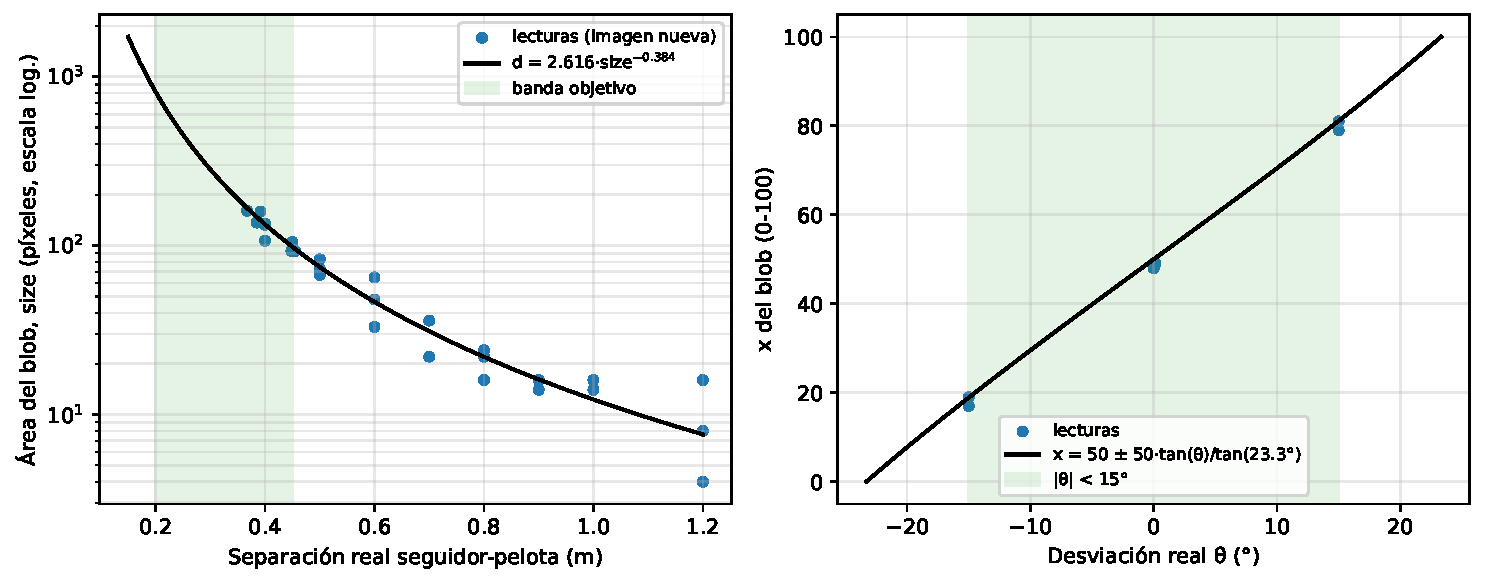
\includegraphics[width=\linewidth]{caracterizacion.pdf}
\caption{Caracterización del detector. Izquierda: tamaño del blob frente a la separación real y modelo ajustado.
Derecha: posición horizontal del blob frente al ángulo real de la pelota.}
\label{fig:caract}
\end{figure}

\begin{figure}[h]
\centering
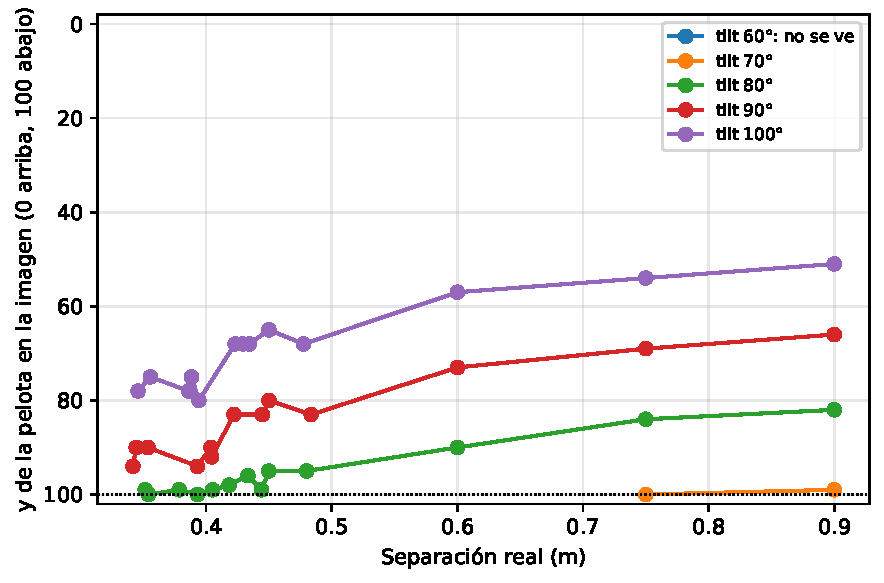
\includegraphics[width=0.55\linewidth]{barrido_tilt.pdf}
\caption{Altura de la pelota en la imagen según la inclinación de la cámara. Con 100 grados se ve en todo el rango
que interesa.}
\label{fig:tilt}
\end{figure}

\begin{figure}[p]
\centering
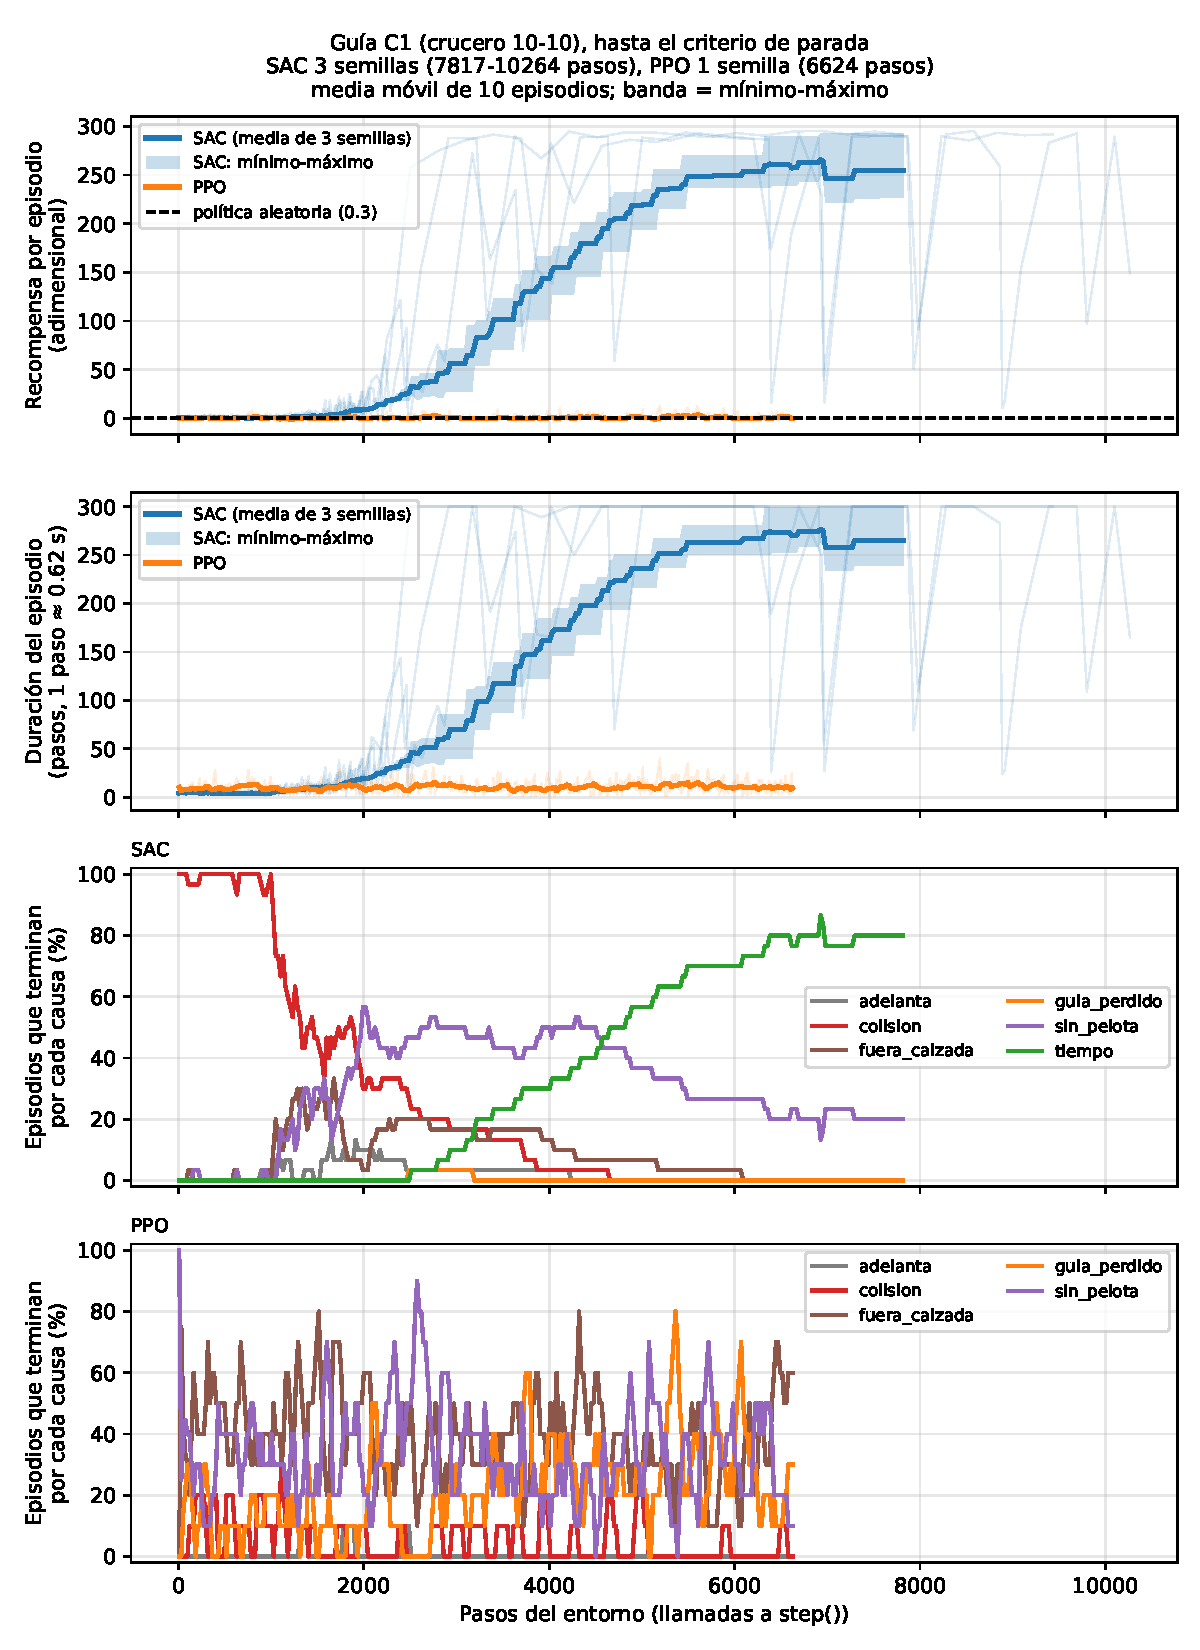
\includegraphics[height=0.85\textheight]{curvas_C1.pdf}
\caption{C1 (crucero 10-10): SAC con 3 semillas (media y banda entre mínimo y máximo, 7817 a 10264 pasos) y PPO
con 1 semilla (6624 pasos).}
\label{fig:C1}
\end{figure}

\begin{figure}[p]
\centering
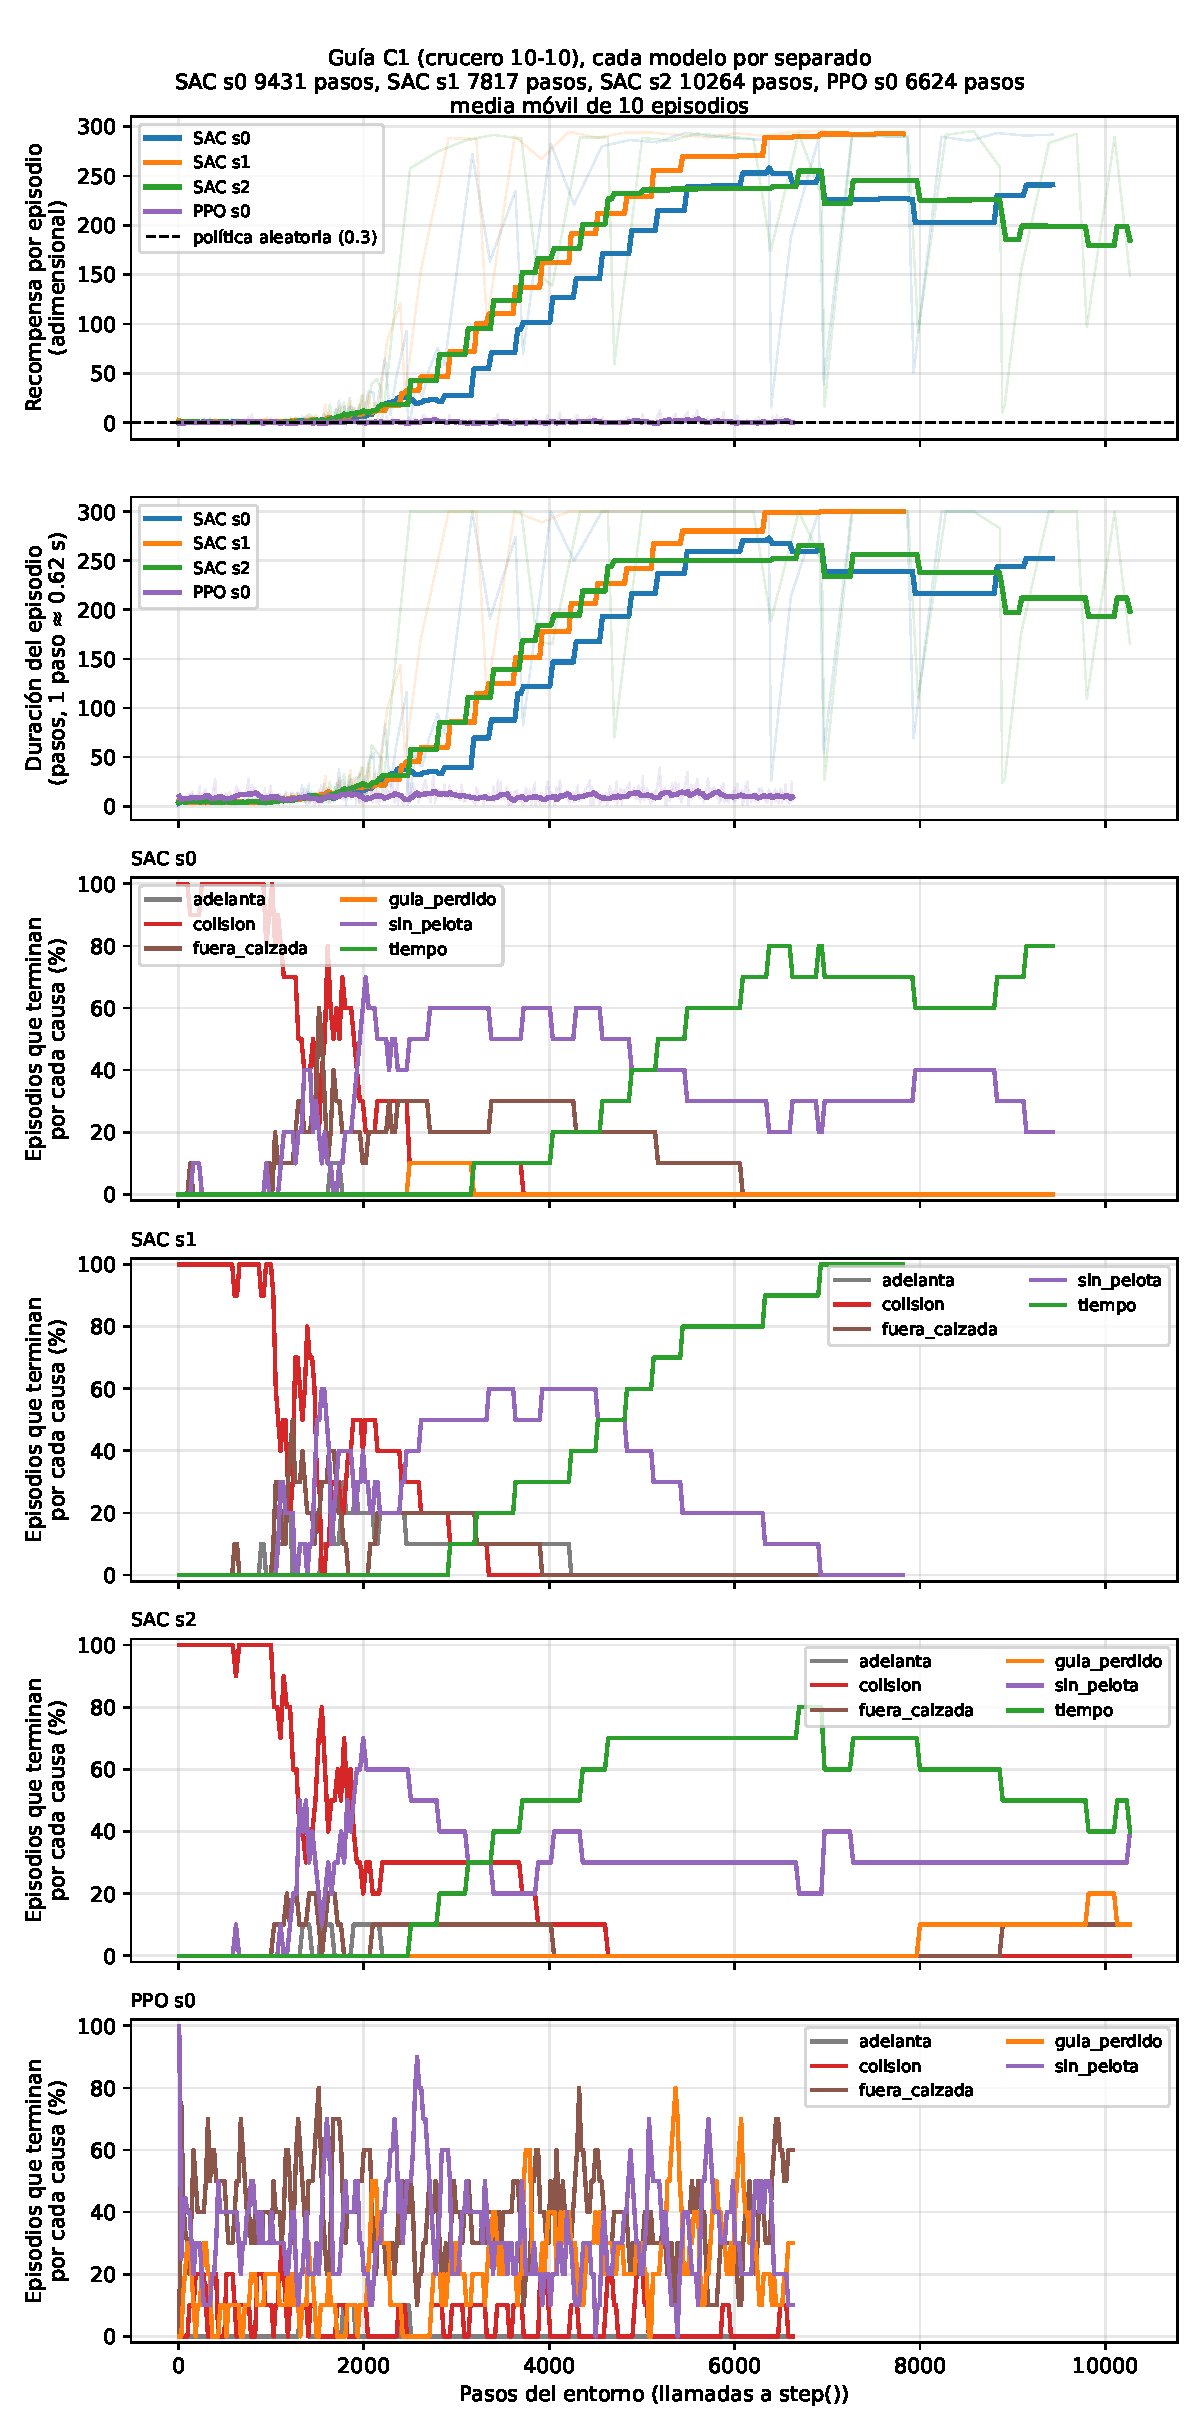
\includegraphics[height=0.85\textheight]{curvas_C1_modelos.pdf}
\caption{C1, cada modelo por separado.}
\label{fig:C1mod}
\end{figure}

\begin{figure}[p]
\centering
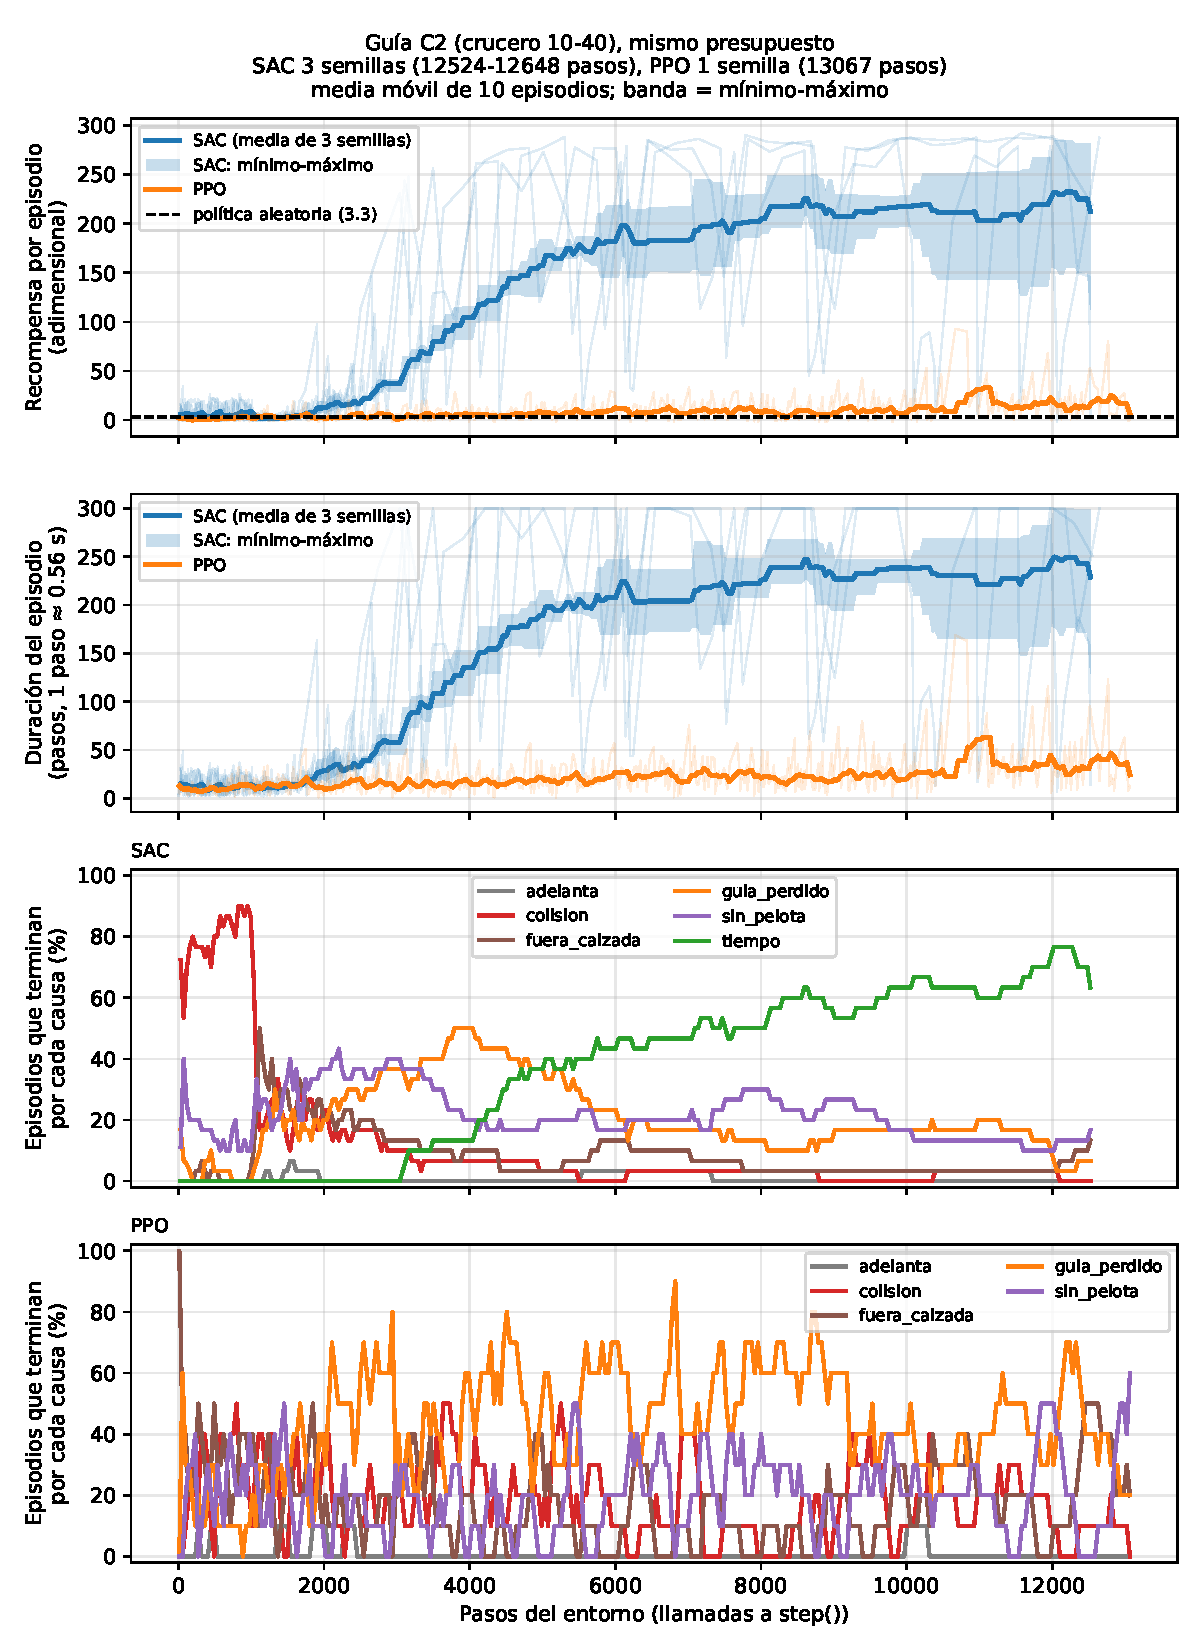
\includegraphics[height=0.85\textheight]{curvas_C2.pdf}
\caption{C2 (crucero 10-40) con el mismo número de pasos: SAC con 3 semillas (12524 a 12648 pasos) y PPO con 1
semilla (13067 pasos).}
\label{fig:C2}
\end{figure}

\begin{figure}[p]
\centering
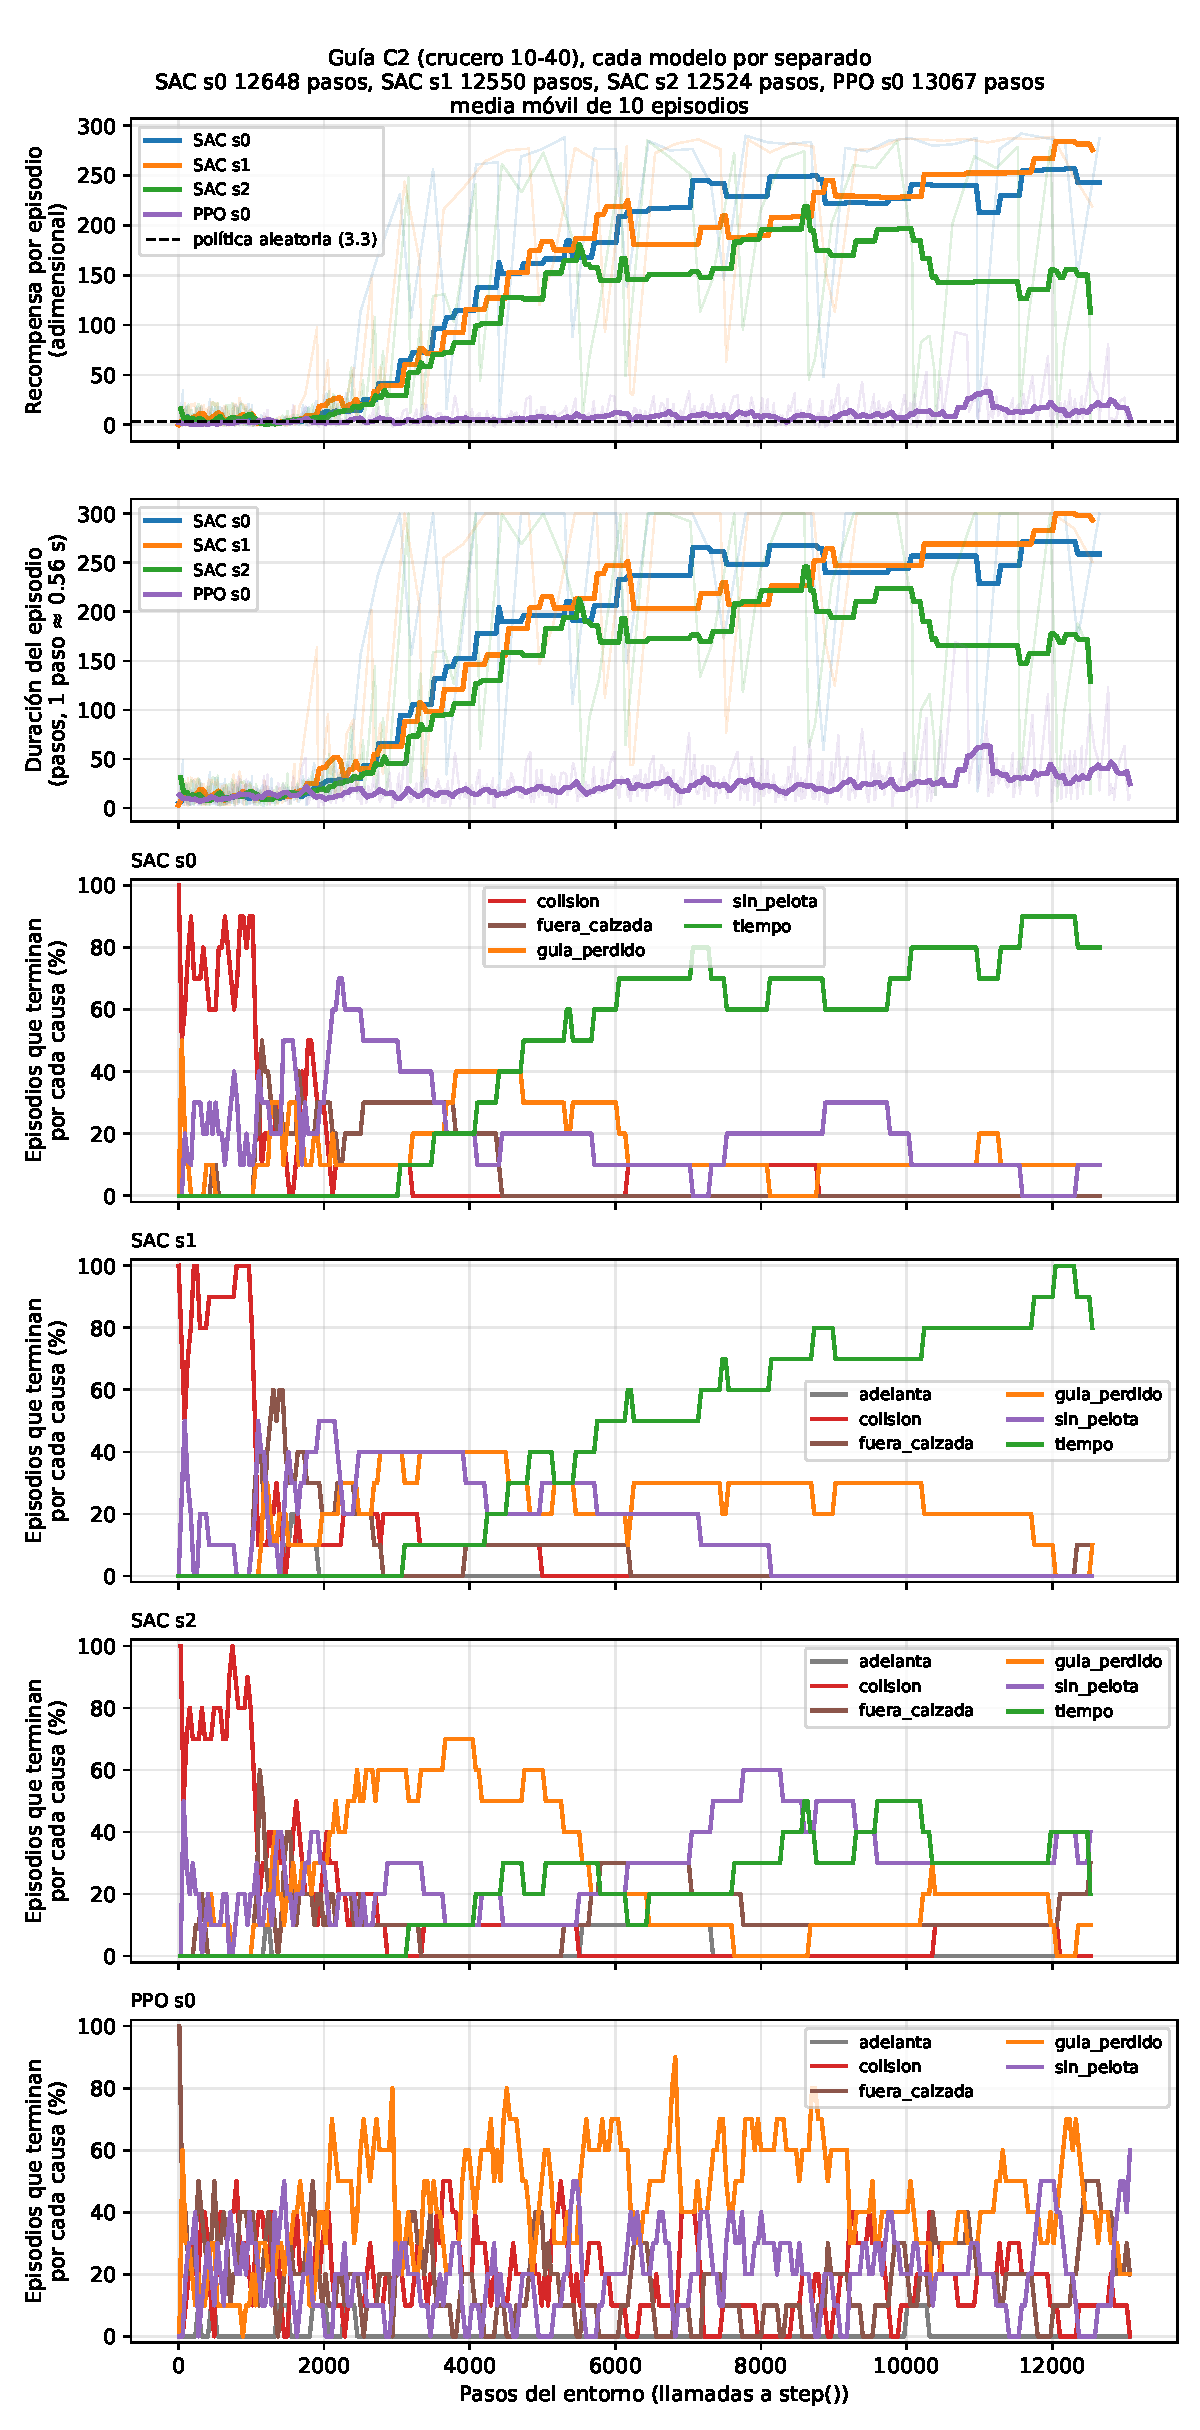
\includegraphics[height=0.85\textheight]{curvas_C2_modelos.pdf}
\caption{C2, cada modelo por separado.}
\label{fig:C2mod}
\end{figure}

\begin{figure}[p]
\centering
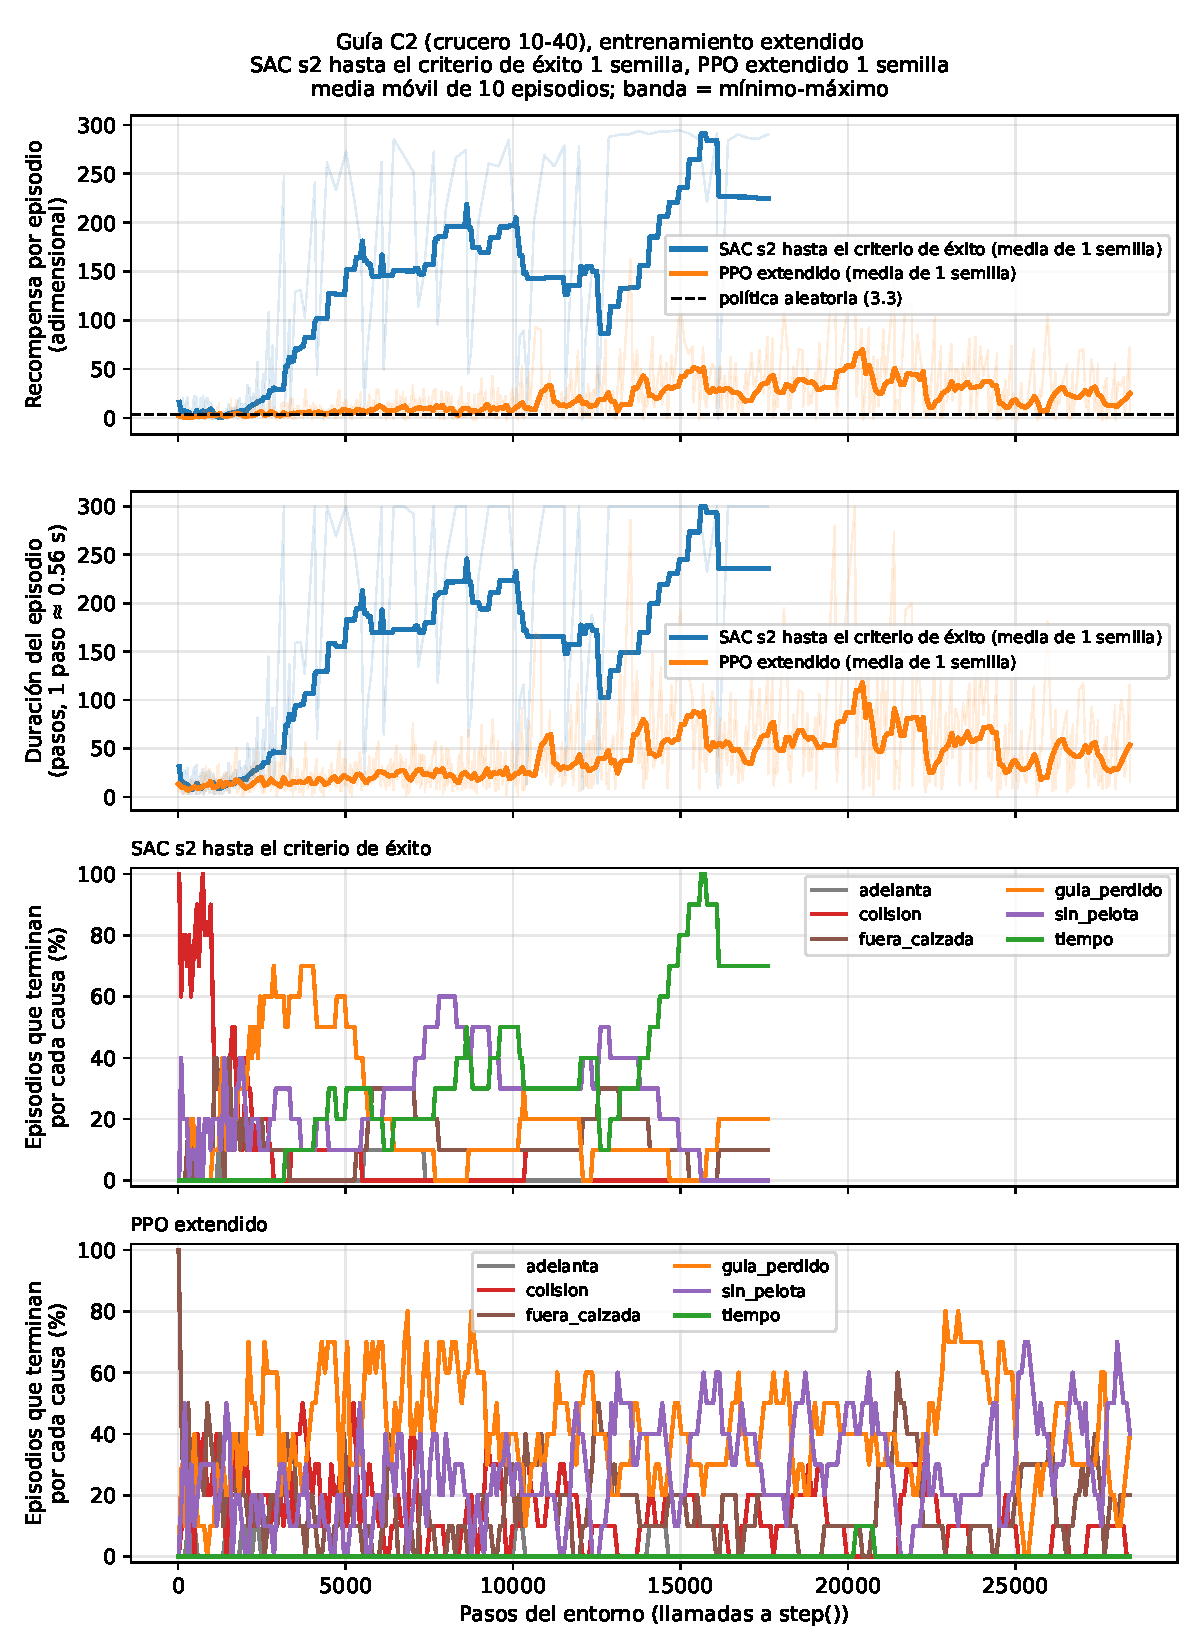
\includegraphics[height=0.85\textheight]{curvas_C2_ext.pdf}
\caption{C2, entrenamientos alargados: SAC s2 hasta el criterio de éxito (17616 pasos) y PPO (28421 pasos).}
\label{fig:C2ext}
\end{figure}

\begin{figure}[p]
\centering
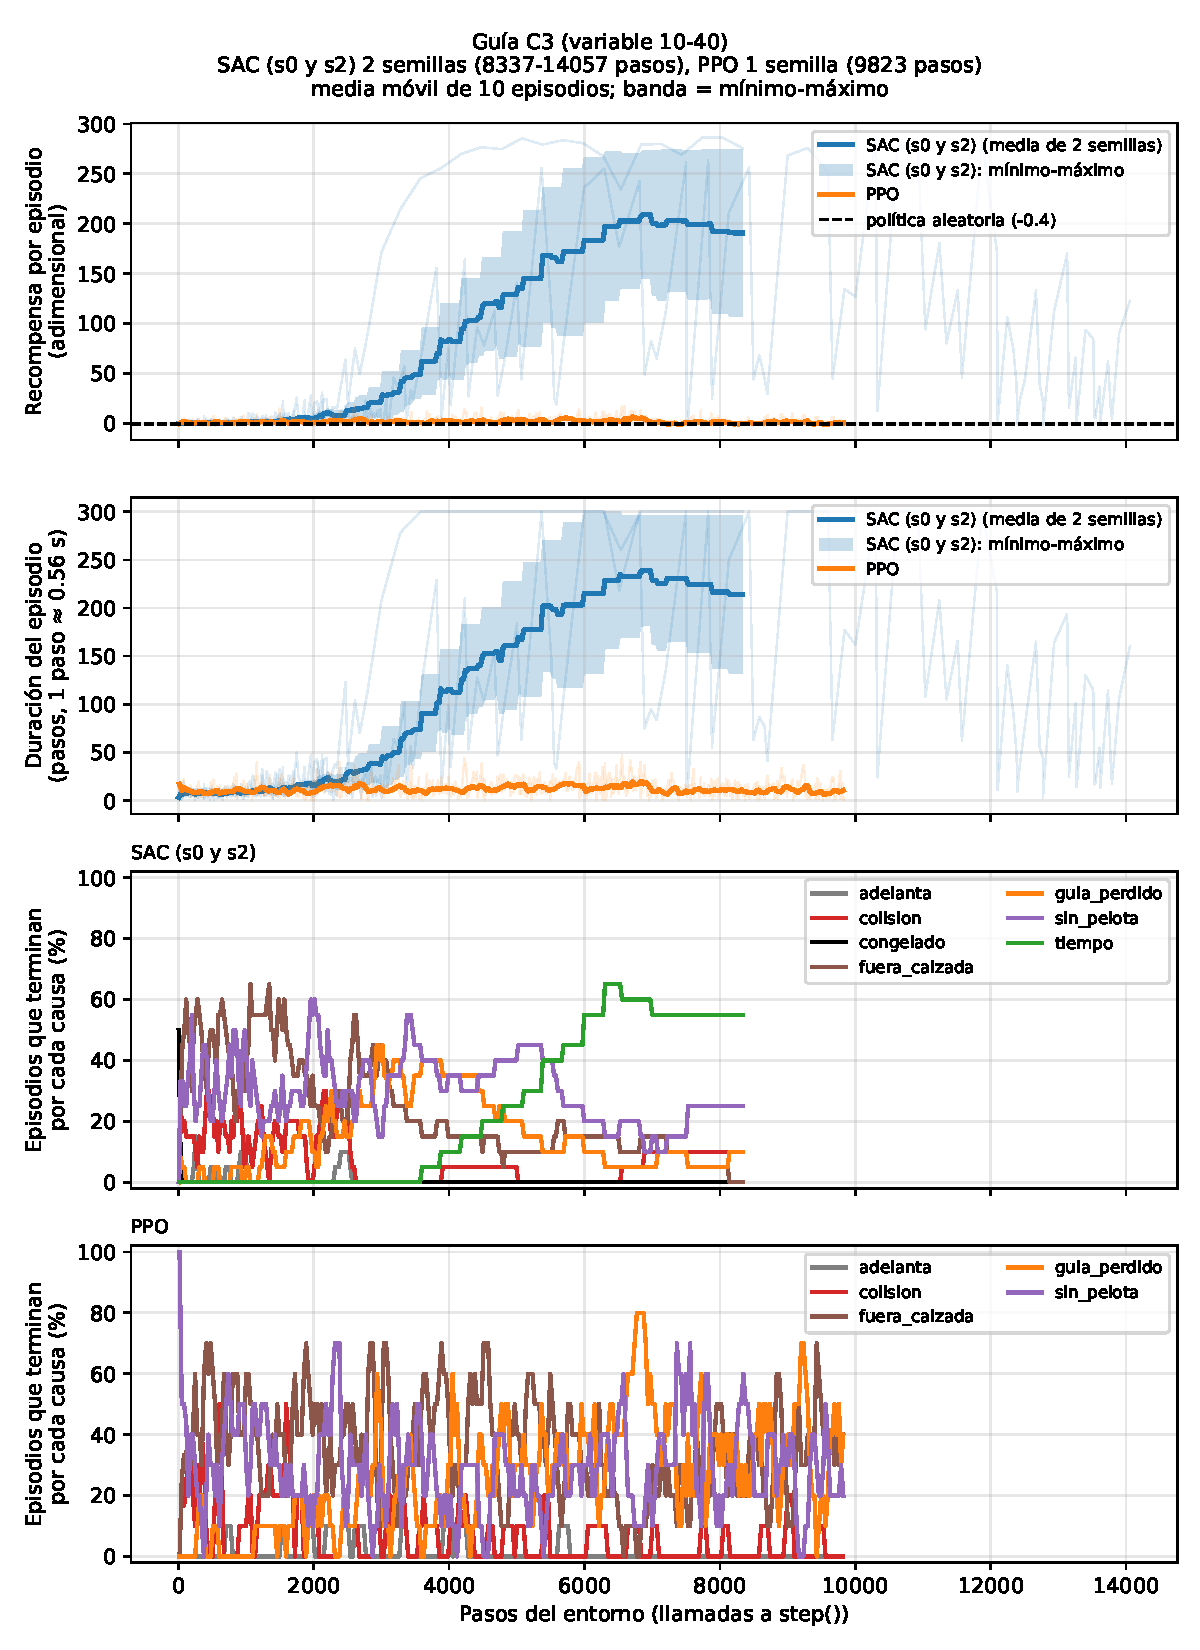
\includegraphics[height=0.85\textheight]{curvas_C3.pdf}
\caption{C3 (variable 10-40): SAC con 2 semillas (s0 y s2, 8337 a 14057 pasos) y PPO con 1 semilla (9823 pasos).
La semilla 1 se deja fuera por el fallo de percepción explicado en el apartado 4.3.}
\label{fig:C3}
\end{figure}

\begin{figure}[p]
\centering
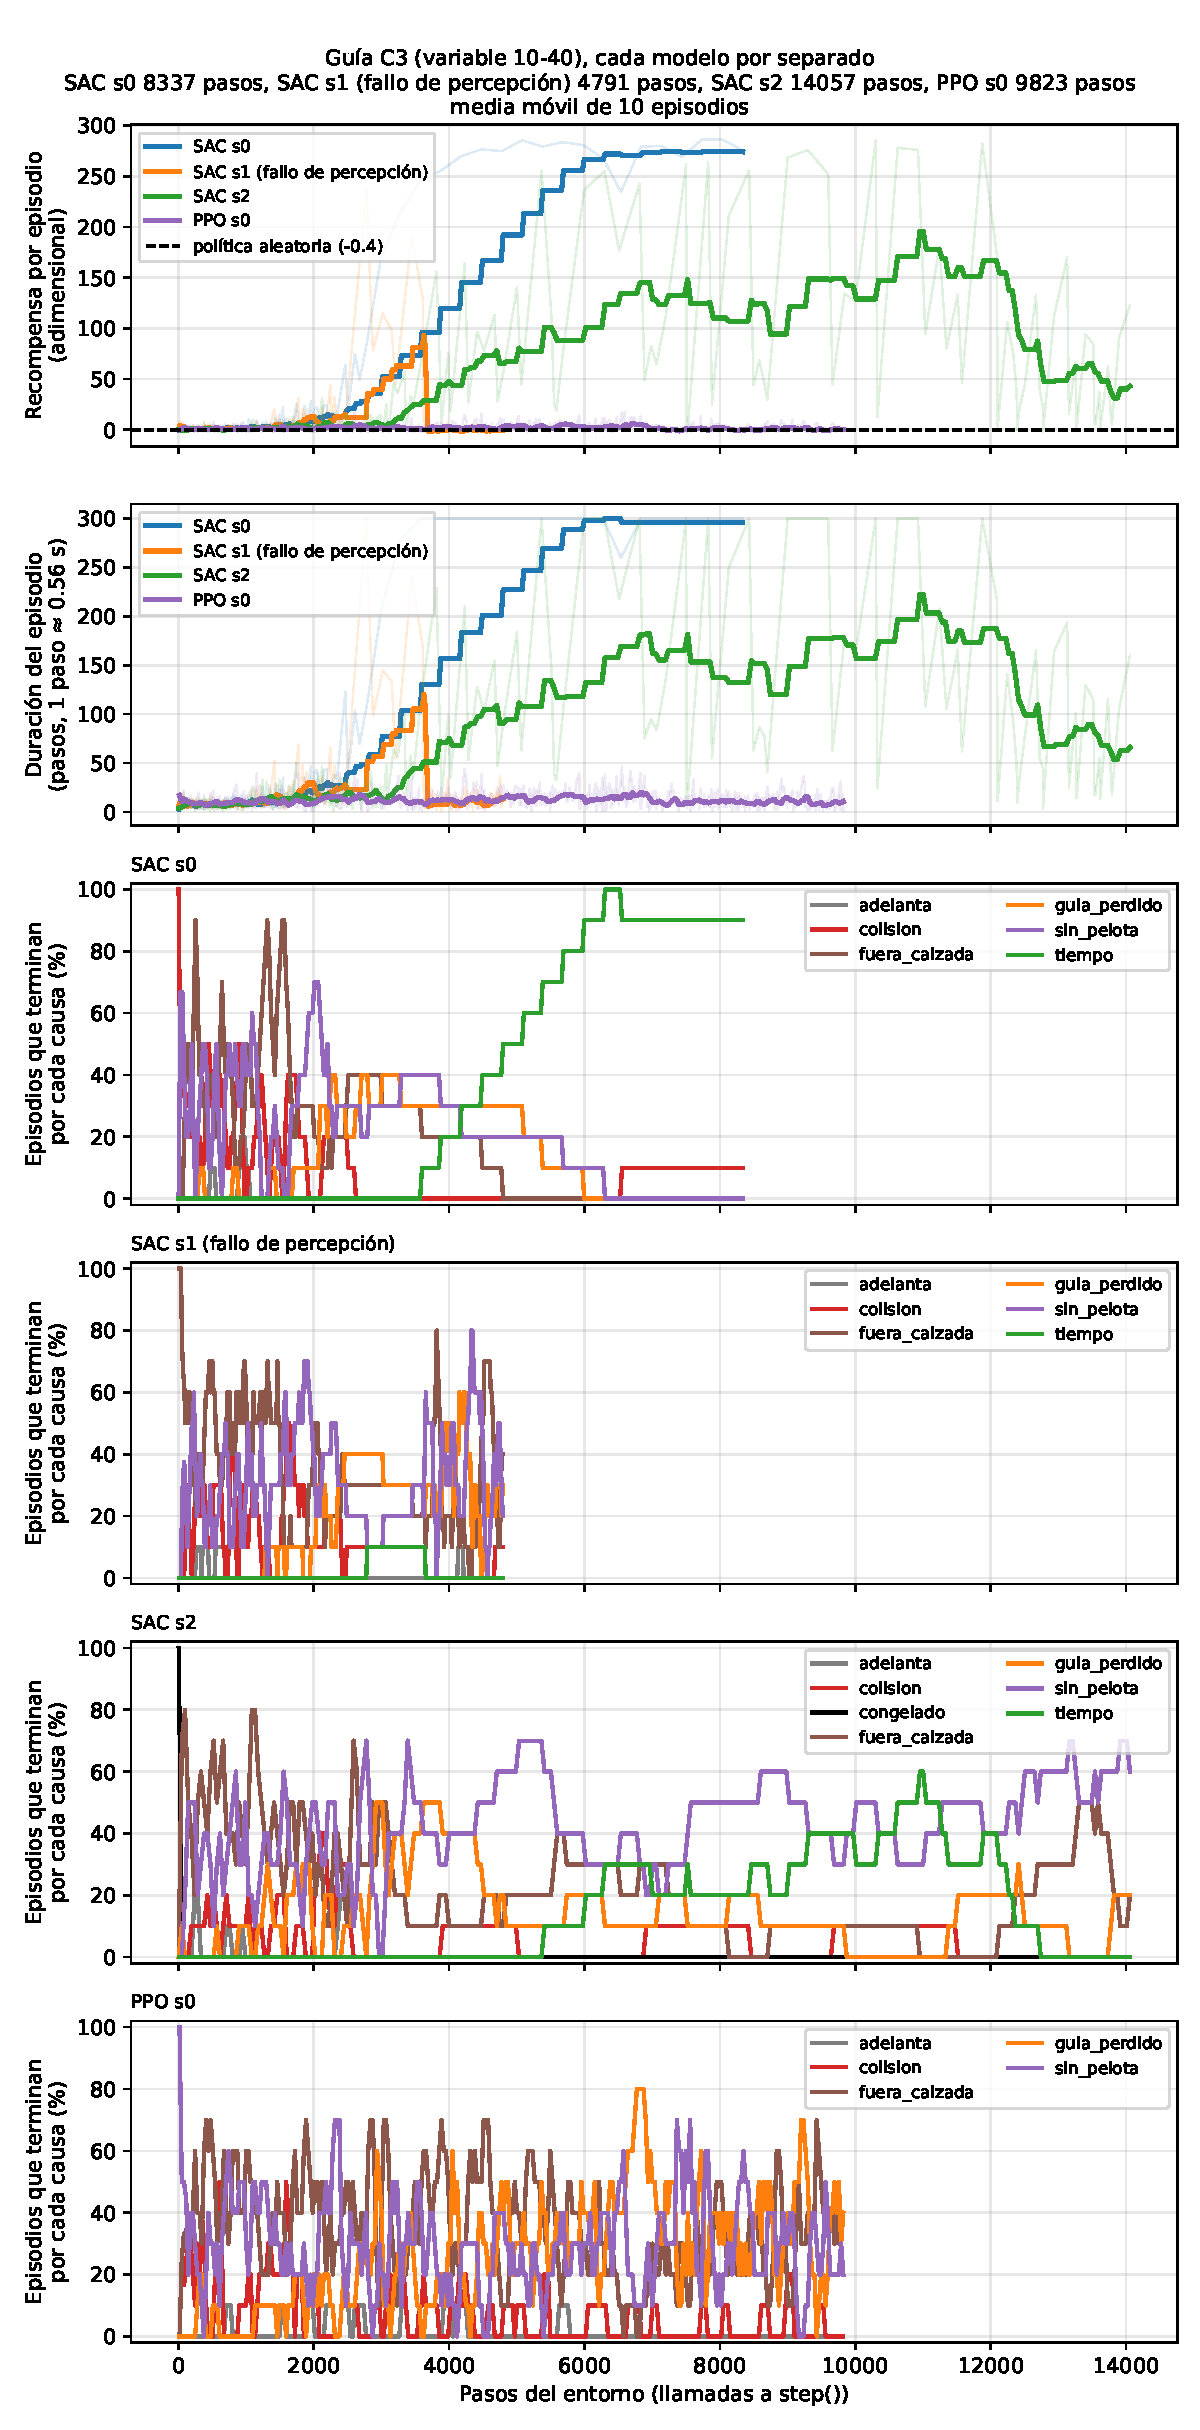
\includegraphics[height=0.85\textheight]{curvas_C3_modelos.pdf}
\caption{C3, cada modelo por separado. En SAC s1 se ve la caída brusca hacia el paso 3615 por el fallo de
percepción.}
\label{fig:C3mod}
\end{figure}

\end{document}
